\documentclass[12pt]{article}
%\usepackage{xltxtra}
\usepackage{fancyhdr}
\usepackage{graphicx}
\usepackage{subcaption}
\usepackage{enumerate}
\usepackage{amsmath}
\usepackage{amssymb, bm}
\usepackage{hyperref}
\hypersetup{ %
	colorlinks=true,
    linkcolor=blue, %mydarkblue,
    citecolor=blue, %mydarkblue,
    filecolor=blue, %mydarkblue,
    urlcolor=blue, %mydarkblue,
} 
%\usepackage[utf8]{inputenc}
%\usepackage[T1]{fontenc}
%\usepackage{fontspec}
%\usepackage{xunicode}

\newcommand{\iid}{\stackrel{\text{iid}}{\sim}}
\newcommand{\eqInDist}{\stackrel{\text{d}}{=}}

\newcommand{\mysec}[1]{Section~\ref{sec:#1}}
\newcommand{\eq}[1]{Eq.~(\ref{eq:#1})}
\newcommand{\myfig}[1]{Figure~\ref{fig:#1}}

\newcommand{\BEAS}{\begin{eqnarray*}}
\newcommand{\EEAS}{\end{eqnarray*}}
\newcommand{\BEA}{\begin{eqnarray}}
\newcommand{\EEA}{\end{eqnarray}}
\newcommand{\BEQ}{\begin{equation}}
\newcommand{\EEQ}{\end{equation}}
\newcommand{\BIT}{\begin{itemize}}
\newcommand{\EIT}{\end{itemize}}
\newcommand{\BNUM}{\begin{enumerate}}
\newcommand{\ENUM}{\end{enumerate}}
\newcommand{\BA}{\begin{array}}
\newcommand{\EA}{\end{array}}
\newcommand{\diag}{\mathop{\rm diag}}
\newcommand{\var}{\mathop{\rm var}}
\newcommand{\mean}{\mathop{\rm mean}}
\newcommand{\Diag}{\mathop{\rm Diag}}

\newcommand{\nn}{\nonumber}
\newcommand{\half}{\frac{1}{2}}
\newcommand{\1}{{\bf 1}}
\newcommand{\st}{\text{ s.t.}}
\newcommand{\ie}{\text{ i.e.}}
\newcommand{\rb}{\mathbb{R}}
\newcommand{\cb}{\mathbb{C}}
\newcommand{\zb}{\mathbb{Z}}
\newcommand{\tr}{{\rm tr}}
\newcommand{\idm}{I}
\newcommand{\BlackBox}{\rule{1.5ex}{1.5ex}}  % end of proof
\newcommand{\indep}{\bot\!\!\!\bot}

\newcommand{\E}{\mathbb{E}}

\newenvironment{proof}{\par\noindent{\bf Proof\ }}{\hfill\BlackBox\\[2mm]}

\newtheorem{proposition}{Proposition}
\newtheorem{lemma}{Lemma}


% If your paper is accepted, change the options for the package
% aistats2e as follows:
%
%\usepackage[accepted]{aistats2e}
%
% This option will print headings for the title of your paper and
% headings for the authors names, plus a copyright note at the end of
% the first column of the first page.
\setlength{\parindent}{0cm}
%\ifMain
\addtolength{\oddsidemargin}{-2cm}
\addtolength{\evensidemargin}{-2cm}
\setlength{\textwidth}{17.78cm}
\addtolength{\topmargin}{-2.7cm}
\setlength{\textheight}{24.24cm}
%\else
\addtolength{\parskip}{5mm}
%\fi
\pagestyle{fancy}

\title{Hwk 5}
\author{Simon Lacoste-Julien}

\begin{document}
\fancyhead{}
\fancyfoot{}

\fancyhead[R]{
  \begin{tabular}[b]{l}
    Name: \hspace{3cm} \\
    Student id: \hspace{3cm} \\
  \end{tabular}
  %\vspace*{10\baselineskip}
}
\fancyhead[L]{
  \begin{tabular}[b]{l}
    IFT6269-A2018  \\
    Prof: Simon Lacoste-Julien \\
  \end{tabular}
  %\vspace*{10\baselineskip}
}
\fancyhead[C]{
  \begin{tabular}[b]{c}
    {\bf Hwk 5} \\
    Due date: Dec 11, 2018
  \end{tabular}
}

%\vspace{0.3cm}

As usual, please hand in on paper form your derivations and answers to the questions. You can use any programming language for your source code (submitted on Studium as per the website instructions). All the requested figures should be printed on paper with clear titles that indicate what the figures represent.

\begin{enumerate}
\item {\bf Cautionary tale about importance sampling (10 points)} \\
Suppose that we wish to estimate the normalizing constant $Z_p$ for an un-normalized Gaussian $\tilde{p}(x) = \exp(-\frac{1}{2\sigma_p^2} x^2)$; i.e. we have $p(\cdot) \sim \mathcal{N}(0,\sigma_p^2)$ with $p(x) = \tilde{p}(x)/Z_p$. Given $N$ i.i.d. samples $x^{(1)},\ldots, x^{(N)}$ from a standard normal $q(\cdot) \sim \mathcal{N}(0,1)$, consider the importance sampling estimate:
$$
\hat{Z} = \frac{1}{N} \sum_{i=1}^N \frac{\tilde{p}(x^{(i)})} {q(x^{(i)})}.
$$
\begin{enumerate}
\item Show that $\hat{Z}$ is an unbiased estimator of $Z_p$.
\item Letting $f(x) := \tilde{p}(x)/q(x)$, show that $\text{var}(\hat{Z}) = \frac{1}{N} \text{var}(f(X)))$ whenever $\text{var}(f(X))$ is finite.
\item For what values of $\sigma_p^2$ is this variance actually finite?
\end{enumerate}


\vspace{1cm}
\item {\bf Gibbs sampling and mean field variational inference (30 points)} \\
Consider the Ising model with binary variables $X_s \in \{0,1\}$ and a factorization of the form:
$$
p(x; \eta) = \frac{1}{Z_p} \exp \left( \sum_{s \in V} \eta_s x_s + \sum_{\{s,t\} \in E} \eta_{st} x_s x_t \right).
$$
We consider the $7 \times 7$ 2D grid as shown in Figure~\ref{fig:grid} (note that we used toroidal (donut-like) boundary conditions to make the problem symmetric). We will consider approximate inference methods to approximate the node marginal moments $\mu_s := p(X_s = 1)$ in this model.

\begin{enumerate}
\item Derive the Gibbs sampling updates for this model. Implement the algorithm (with cyclic sequential traversal of the nodes) for $\eta_{st} = 0.5$ for all edges, and $\eta_s = (-1)^s$ for all $s \in \{1, \ldots, 49\}$ (using the node ordering of Figure~\ref{fig:grid}). Run a burn-in period of 1000 epochs (where one epoch amounts to updating each node once). For each of the 5000 subsequent epochs, collect a sample vector, and use the 5000 samples to form Monte Carlo estimates $\hat{\mu}_s$ of the moments $\E[X_s]$ at each node.\footnote{Note that I said in class that every update of a node yields a \emph{different} sample in theory, and that one should normally use \emph{all} the available samples (after sufficient mixing) for a Monte Carlo estimate, i.e. here it would be $49 \times 5000$ samples. But note that using all these samples would give almost the exact same estimates, only differing from the boundary conditions during the first and last epoch...}
Output a $7 \times 7$ matrix of the estimated moments.
Repeat the experiment $10$ times and output a $7 \times 7$ matrix of the empirical standard deviation of your estimate at each node (this gives an idea of the variability of your estimates).

\item Derive the naive mean field updates (based on a fully factorized approximation), where we use the notation $q(X_s =1) = \tau_s$, and implement them for the same model. More specifically, do cyclic coordinate descent on $KL(q || p)$, sequentially updating the parameter $\tau_s \in [0,1]$ for $s=1, \ldots, 49$. Derive the expression for $KL(q || p)-\log(Z_p)$ and plot it as a function of the number of epochs both for debugging purpose and monitor progress. Let $d(\tau, \tau'):= \frac{1}{49} \sum_{s=1}^{49} |\tau_s - \tau'_s|$ be the average $\ell_1$ distance between two parameters. Use $d(\tau^{(k-1)}, \tau^{k}) <  0.001$ as a stopping criterion for convergence (where $k$ counts the number of epochs). Compute $d(\hat{\tau}_s, \hat{\mu}_s)$ between the mean field estimated moments $\hat{\tau}_s$ and the Gibbs estimates $\hat{\mu}_s$.  Is the mean field a good approximation here? Try different initializations -- does it get stuck in different local minima?

\end{enumerate}

\begin{figure}
\centering
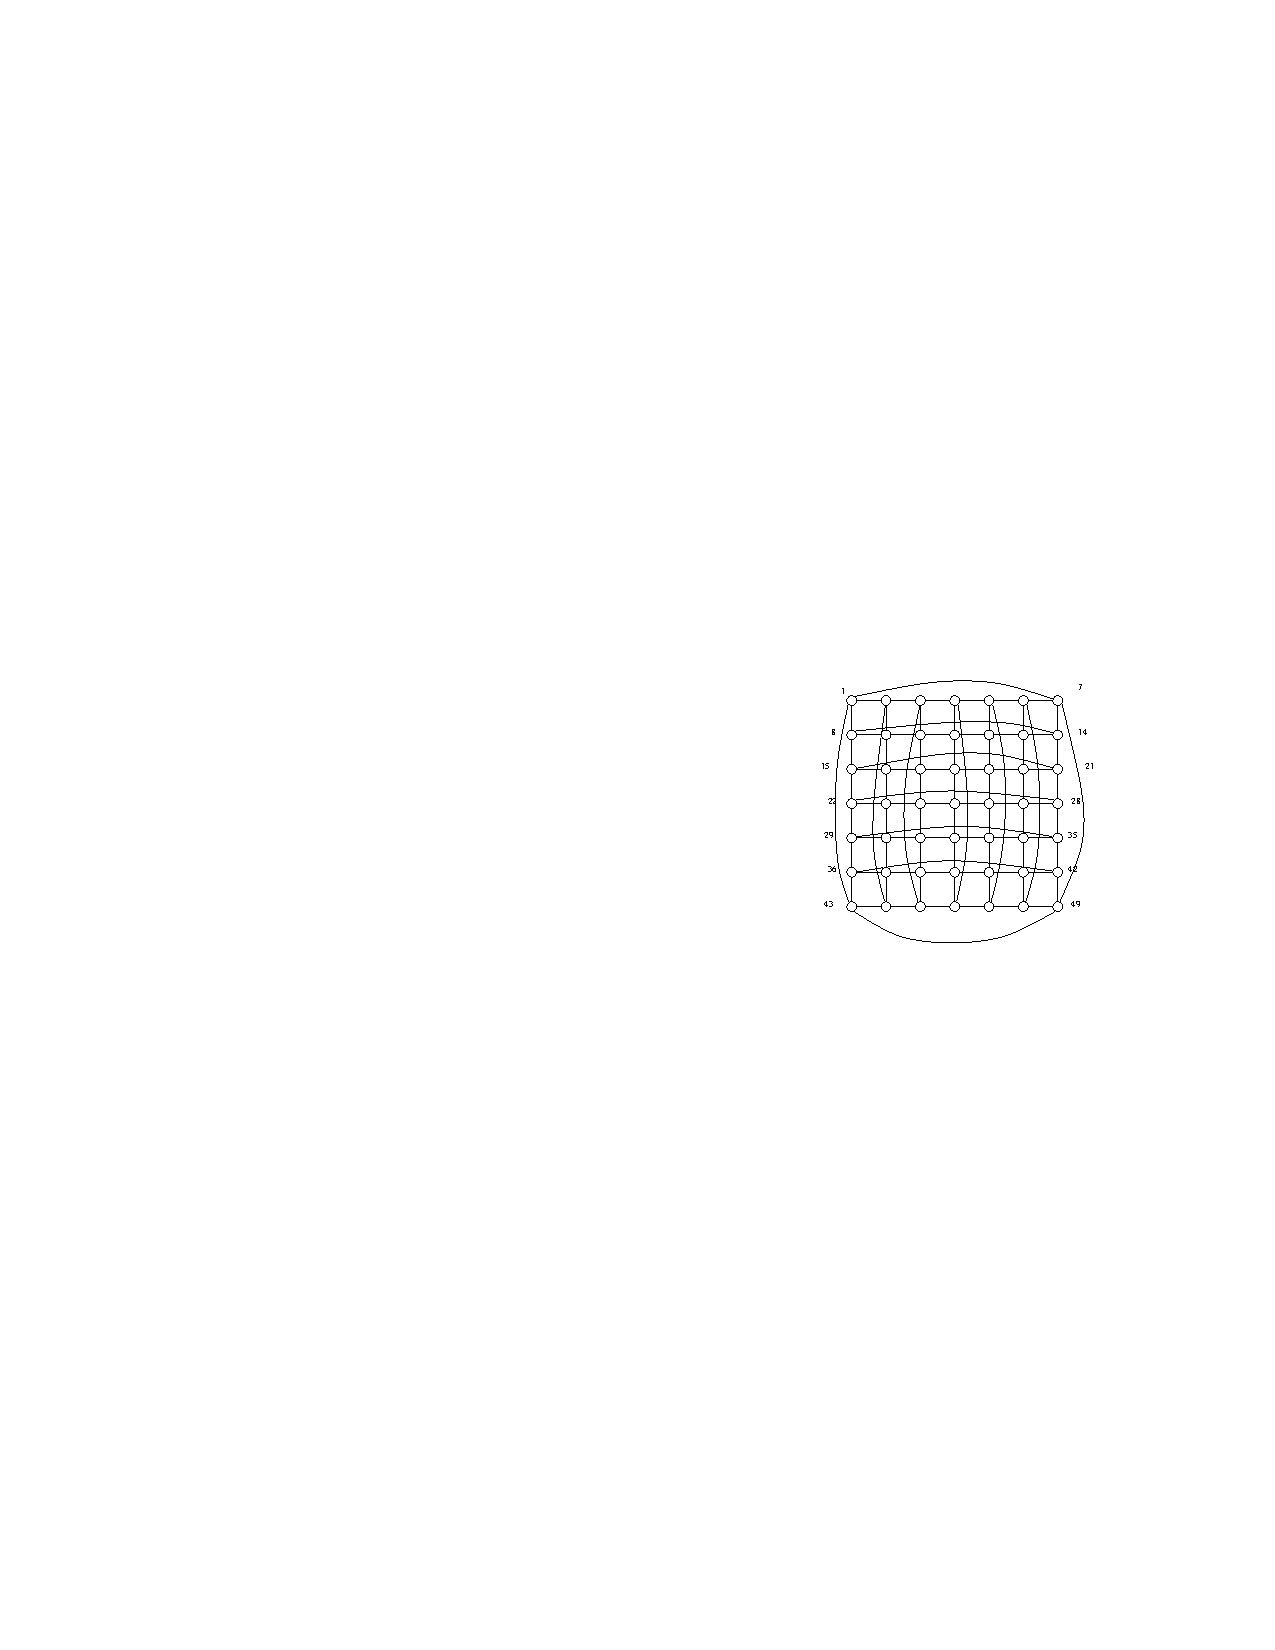
\includegraphics[scale=1.5]{grid.pdf}
\caption{The undirected graphical model considered. \label{fig:grid}}
\end{figure}

\end{enumerate}

\end{document}


